% Chapter 1
\stepcounter{cap}
%\chapter{cap1}
\label{cap2}

\mychapter{2}{Capitolul \arabic{cap} \\ BAZA DE DATE}
%\chapter{\arabic{cap}.Introducere} % Main chapter title

\label{Chapter2} % For referencing the chapter elsewhere, use \ref{Chapter1} 

\thispagestyle{fancy}

%-----------------------------------------------------------------
\section{Alegerea tipului de bază de date} 
	Nevoia modulului de a stoca şi de a accesa datele stocate anterior a dus la realizarea unui mic studiu în vederea alegerii tipului de bază de date cel mai potrivit.

	\subsection{Factori de decizie} 
	\begin{itemize}
	 \setlength\itemsep{0em}
		\item Consistenţa datelor stocate
		\item Utilizarea RAM-ului
		\item Timp de accesare la pornirea aplicaţiei
		\item Timp de accesare în cadrul aplicaţiei
		\item Spaţiul ocupat pe disc
		\item Compatibilitate cu versiunile anterioare
	\end{itemize}

	\subsection{Soluţii propuse}
	În următorul tabel, se presupune ca pentru fişierele binare, XML şi JSON este necesară încărcarea datelor la pornirea aplicaţiei. SQLite oferă însă soluţii de căutare inteligente, nefiind necesară încărcarea tuturor datelor la pornirea aplicaţiei.

	\begin{table}
	\caption{Compararea principalelor metode de stocare a datelor pe baza factorilor de influenţare}
	\resizebox{\textwidth}{!}{\begin{tabular}{ | c | c | c | c | c |}
	\hline
		& \textbf{Binar} & \textbf{XML sau JSON} & \textbf{SQLite} & \textbf{Memorare în Cloud} \\ 
	\hline
	 Consistenţa datelor stocate & Nu & Nu & Da & Da \\
	\hline
	 Utilizarea RAM-ului & Ridicat & Scăzut & Mediu & Mediu \\
	\hline
	 Timp de accesare la pornirea aplicaţiei & Mediu & Ridicat & Scăzut & Scăzut \\
	\hline
	 Timp de accesare în cadrul aplicaţiei & Scăzut & Scăzut & Mediu & Ridicat \\
	\hline
	 Spaţiul ocupat pe disc & Scăzut & Ridicat & Scăzut & Foarte scăzut \\
	\hline
	 Compatibilitate cu versiunile anterioare & Nu & Da & Da & Nu \\
	\hline
	\end{tabular}}
	\end{table}

	\subsection{Soluția aleasă}
	S-a decis folosirea SQLite ca format pentru baza de date deoarece îndeplinea toate criteriile specificate.


\section{Structura bazei de date}


\begin{figure}[h!]
  \centering
    \centering{%
      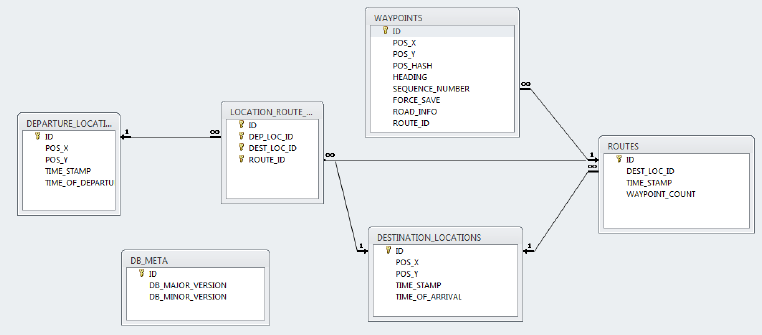
\includegraphics[width=0.9\textwidth]{Figures/baza_date.png}}
  \caption{Structura tabelelor de date şi relaţiile dintre ele}
\end{figure}

Tabelele din figura de mai sus sunt folosite pentru realiza structura întregii baze de date.
\vspace{6pt}
\\Tabela meta este folosită la identificarea versiunii bazei de date. Acest lucru este necesar pentru a detecta compatibilitatea şi pentru a permite migrarea către o versiune mai recentă. 
\vspace{6pt}
\\Datele înregistrate sunt separate în puncte de plecare, destinaţii, rute şi waypoint-uri. O rută este întotdeauna formată din mai multe waypoint-uri, unul sau mai multe puncte de plecare şi una sau mai multe destinaţii. Ruta (waypoint-urile) sunt stocate numai o singură dată, în timp ce toate punctele de plecare şi destinaţiile sunt stocate. În acest fel, numărul de destinaţii poate influenţa probabilitatea rutei.
\vspace{6pt}
\\Accesul la date se face prin SQLite. Toate datele stocate pot fi atât citite cât şi modificate.


